\documentclass[a4paper,11pt]{article}
\usepackage{style}

\begin{document}

\fiche{NP-Complétude}
\titre{Diviser pour mieus régner :} Diviser $\rightarrow$ Régner $\rightarrow$ Combiner\\
\titre{Théorème Maître:} 
\begin{itemize}
	\item Si $f(n) = O(n^{\mathrm{log}_ba-\varepsilon})$ ($\varepsilon > 0)$ alors $T(n)\in O(n^{\mathrm{log}_ba})$
	\item Si $f(n) = \theta(n^{\mathrm{log}_ba})$ alors $T(n) = O(n^{\mathrm{log}_ba}\ln n)$
	\item Si $f(n) = \Omega(n^{\mathrm{log}_ba+\varepsilon})$ ($\varepsilon > 0$) et $\exist c < 1$ tel que $cf(n) > af(\frac{n}{b})$. Alors $T(n) \in O(f(n))$
\end{itemize}
\titre{Programmation dynamique :} Mémoriser les solutions aux sous problèmes pour pouvoir les réutiliser dans le calcul de la solution. \\
\titre{Th :} $T(n) = aT(n-b) + f(n)$, avec $a\geq 2, b\geq 1, f(n) \in \Omega(1)$. Alors $\exist c = \displaystyle{^b\sqrt{a}} > 1 \tq T(n) \in \Omega(c^n)$\\
\titre{BackTrack :} progresse vers une solution en faisant des choix plus ou moins arbitraires et qui revient en arrière lorsqu'il est bloqué\\
\titre{Red. Poly. :} $R\ffonc{I_1}{I_2}$, $P_1(I_1) = P_2(I_2)$, $P_1 \leq_p P_2$\\
\titre{Th :} $P_2$ poly $\impl P_1$ poly. $P_1$ non poly $\impl P_2$ non poly. \\
\titre{NP-Complétude (coNP) :} Un problème $P_0$ est NP-Complet si : 
\begin{itemize}
	\item $P_0 \in $ NP ($\exist$ algo de vérification poly)
	\item $P_0$ est NP-Difficile (pour tout problème $P_1 \in $ NP, on a $P_1 \leq_p P_0$) 
\end{itemize}
\titre{Théorème de Cook :} SAT est NP-Complet \\

\fiche{Problèmes}
\titre{Découpe de barres} \\
\titre{Distance de Levenstein} \\
\titre{Impression équilibrée} \\
\titre{Clique :} $\exist$ une clique de taille $k$ dans $G$ ?\\
\titre{Ensembles indépendants :} $\exist$ dans $G$ un ensemble de $k$ sommets sans arête commune ?\\
\titre{Couverture des arêtes :} $\exist$ dans $G$ un ensemble de $k$ sommets tel que toute arête soit adjacente à un sommet de cet ensemble ? \\
\titre{Cycle Hamiltonnien :} $\exist$ un cycle qui passe une et une seule fois par chaque arête. \\
\titre{Problème du voyageur de commerce :} $\exist$ un chemin de taille $\leq k$ passant par tous les sommets ? \\
\titre{Sudoku de taille $N$ :} Grille de $N^2$ lignes, $N^2$ colonnes, $N^2$ blocs de taille $N^2$. Complétez la grille avec des nombres de $1$ à $N^2$. \\
\titre{Couverture exacte :} Etant donnée une matrice binaire $M$ sélectionner $k$ lignes de manière à avoir une et une seule occurence de 1 sur chaque colonne. \\
Solution X de type BackTrack : Pour une colonne donnée, supprimer les lignes contenant 1 sauf une, puis si X(M) alors vrai, sinon annuler la suppression et recommencer. \\
\titre{SAT, 3SAT, CSAT :} Trouver une affectation pour une conjonction de clauses. \\
\titre{Indé $\leq_p$ Clique :} Graphe complémentaire 
\titre{Clique $\leq_p$ Indé :} Graphe complémentaire \\
\titre{CA $\leq_p$ Indé :} $k \rightarrow n-k$ 
\titre{Indé $\leq_p$ Couv :} $k \rightarrow n-k$ \\
\titre{Cycle Hamiltonnien $\leq_p$ Voyageur :} Arête $\rightarrow$ poids 1 ; PasArête $\rightarrow$ poids 2 ; $k = $ nb sommets. \\
\titre{Sudoku $\leq_p$ CE :} $M$ matrice de $N^6$ lignes et $4N^4$ colonnes \\
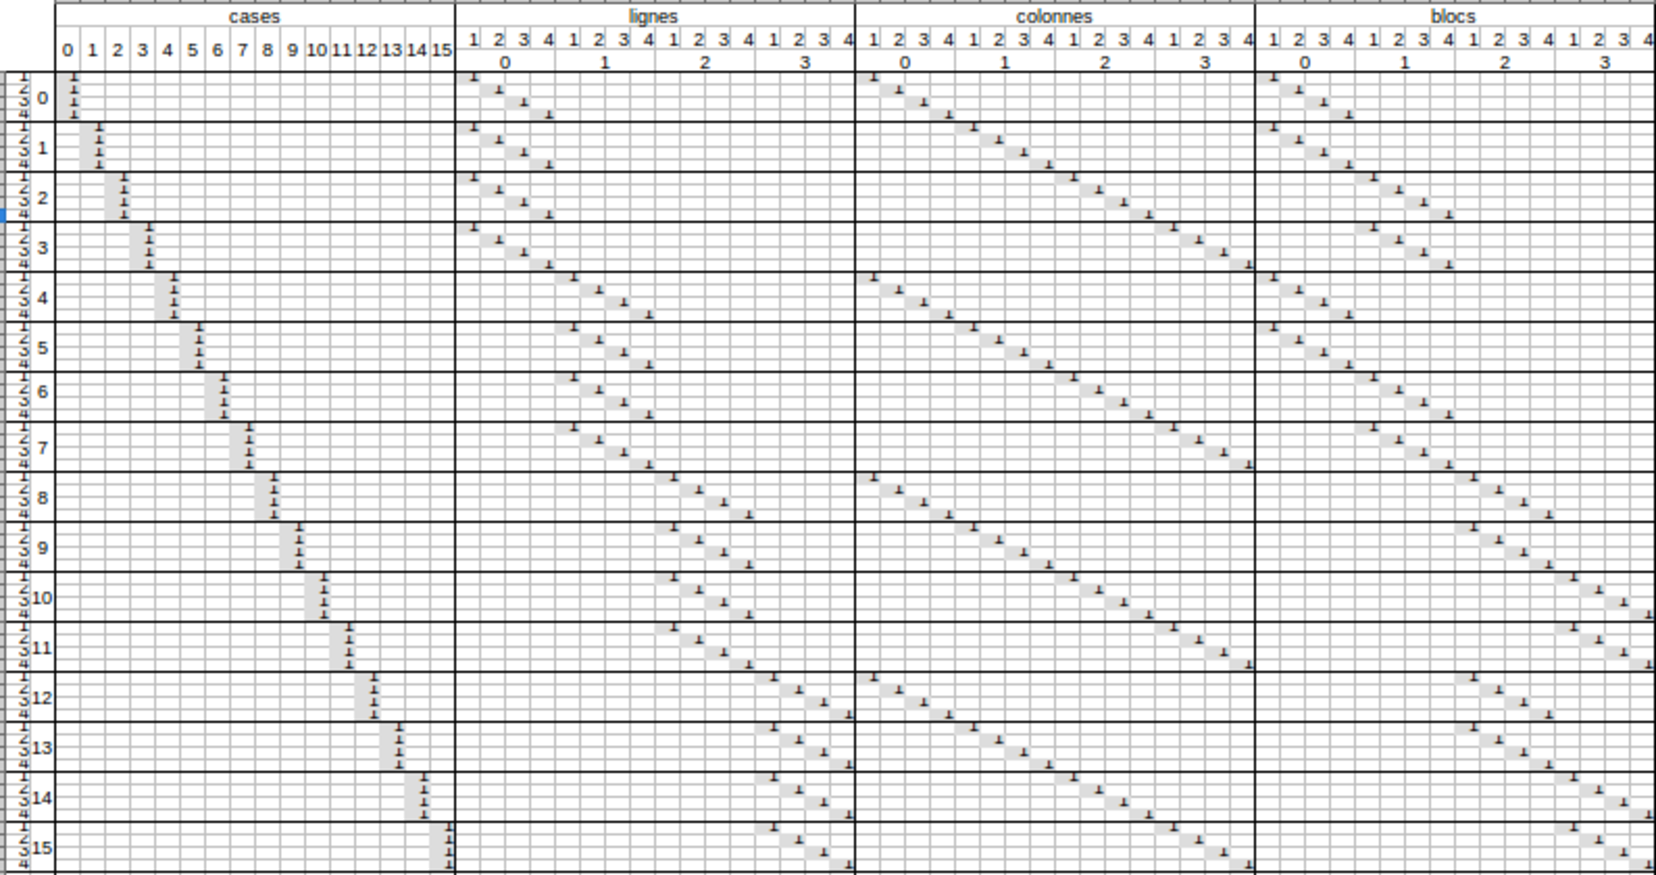
\includegraphics[width=350px]{../Images/04_sudoku_couv.pdf}



\end{document}
